\section{Model inference}
\label{sec:related:modelinf}

In the Industry, software models as defined in
\crossref{sec:related:testing}{sec:related:testing:model} are
often neglected: specifications are not up to date (or even
missing), models are neither accurate nor sound, and also rarely
formals.

Such a situation can be comprehensible because writing complete
documentation and especially formal models is often a tedious and
error prone task. That is why lightweight and incomplete models
are usually found in the Industry. This leads to several issues,
e.g., the toughness of testing applications with a good test
coverage, the difficulty to diagnose failures, or to maintain
models up to date since they are poorly documented.

Solutions to these problems can be initiated by means of model
inference. This research domain originates from works on language
learning started in the 1960s with Gold \cite{Gold1978302}, based
on previous work to formalize natural languages. Model inference
here describes a set of methods that infer a specification by
gathering and analyzing system executions and concisely
summarizing the frequent interaction patterns as state machines
that capture the system's behavior. These models, even if
partial, can be examined by a developer, to refine the
specification, to identify errors, and can be very helpful for
in-depth analysis, etc. Models can be generated from different
kinds of data samples such as affirmative and negative answers
\cite{Angluin198787}, execution traces
\cite{Krka:2010:UDE:1810295.1810324}, documentation
\cite{ZhongZXM11}, source code
\cite{Salah05scenariographer,Pradel:2009}, network traces
\cite{6079839} or from more abstract documentation such as Web
Service Description Language (WSDL)
description \cite{Bertolino:2009:ASB:1595696.1595719}.  Model
inference is employed for different purposes. One can infer
models from log files in order to retrieve important information
in order to identify failure causes \cite{4700316}. It has also
successfully been applied to intrusion detection \cite{debar00},
searching for features in execution traces that allow to
distinguish browsers from other software systems. A prominent use
of model inference also concerns Model-based Testing
\cite{Lorenzoli2008,tap2011,MobiGUITARIEEESoftware2014} and
verification \cite{Ammons:2002:MS:565816.503275}.

In the literature, we can find different techniques to infer
models that can be organized in two main categories. In the first
category, we find the techniques that interact with systems or
humans to extract knowledge that is then studied to build models.
We refer to these methods as active methods. Other works infer
models by assuming that system samples, e.g., a set of traces, is
provided for learning models. We refer to this principle as
passive methods since no interaction is required.

In the following section, we give an overview of prominent active
inference approaches: we introduce $\EuScript{L}^*$-based
techniques in Section \ref{sec:active-letoile}, incremental
learning techniques in Section \ref{sec:active-increment}, and
the model generation by means of automatic testing of
event-driven applications providing Graphical User Interfaces
GUIs) in Section \ref{sec:active-crawling}. Passive inference
techniques are extensively described in Section
\ref{sec:passive}. We cover passive inference techniques using
event sequence-based abstraction in Section
\ref{sec:passive-fsa}, using state-based abstraction in Section
\ref{sec:passive-spec}. Then, we present some white-box
approaches in Section \ref{sec:passive-white}, and we also
mention a few techniques that leverage documentation to infer
models in Section \ref{sec:passive-others}.

%%%%%%%%%%%%%%%%%%%%%%%%%%%%%%%%%%%%%%%%%%%%%%%%%%%%%%%%%%%%%%%%%

\subsection{Active model inference}
\label{sec:active}

\begin{figure}[h]
    \begin{center}
        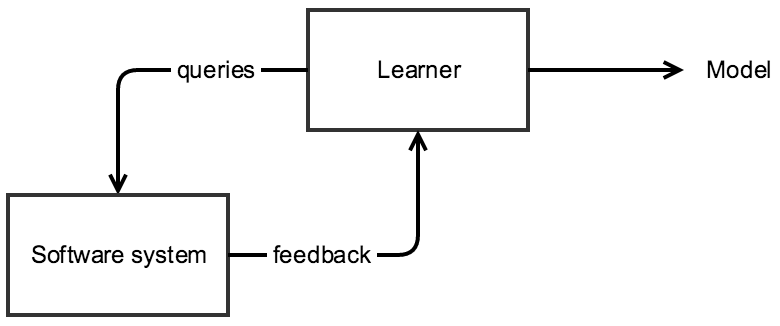
\includegraphics[width=0.9\linewidth]{figures/active.png}
    \end{center}

    \caption{Active model inference principle. Interactions are
        performed with queries that produce feedback a learner
        can use to build a model.}
    \label{fig:active}
\end{figure}

Active inference refers to algorithms that actively interact with
black-box systems or people to extract knowledge about a
(software) system, which is then expressed in a model.
Interactions are performed with kinds of queries, which are
sometimes replaced by testing techniques. A model generator or
learner then uses this feedback to incrementally build several
models, or to refine the model under generation. Many existing
active inference techniques have been initially conceived upon
two concepts: the $\EuScript{L}^*$ algorithm, presented in
Section \ref{sec:active-letoile}, and incremental learning,
presented in Section \ref{sec:active-increment}. Several more
recent papers also proposed crawling techniques of Graphical User
Interface (GUI) applications, i.e. exploring them through their
GUIs with automatic testing. We introduce some of them in Section
\ref{sec:active-crawling}.

\subsubsection{$\EuScript{L}^*$-based techniques and related}
\label{sec:active-letoile}

\begin{figure}[h]
    \begin{center}
        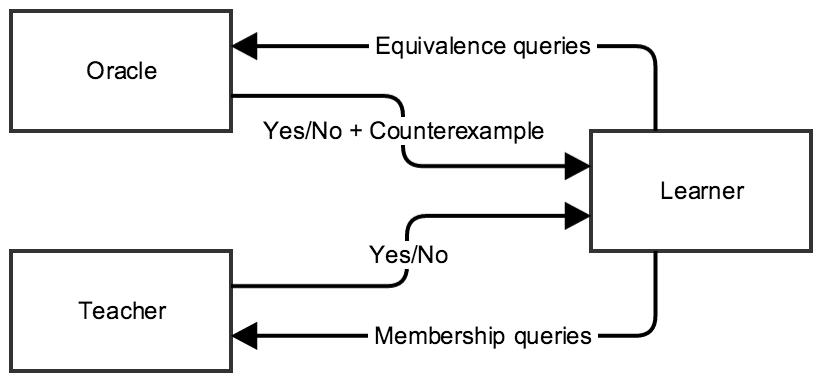
\includegraphics[width=0.9\linewidth]{figures/angluin.png}
    \end{center}

    \caption{The principle of $\EuScript{L}^*$-based learning
    algorithms with two kinds of queries: membership queries and
    equivalence queries.}
    \label{fig:angluin}
\end{figure}

The $\EuScript{L}^*$ algorithm by Angluin \cite{Angluin198787} is
one of the most widely used active learning algorithm for
learning \textit{Deterministic Finite Automata} (DFA). The
algorithm has indeed been applied to various problem domains,
e.g., protocol inference or the testing of circuits. It is
designed to learn a regular language $\EuScript{L}$ by inferring
a minimal DFA $\EuScript{A}$ such that
$\EuScript{L}(\EuScript{A})=\EuScript{L}$, with
$\EuScript{L}(\EuScript{A})$ the set of strings of $\EuScript{A}$
leading to one of its states from its initial one. The algorithm,
also known as the \textit{learner}, knows nothing about
$\EuScript{A}$ except its input alphabet. It relies on two roles,
a \textit{teacher}, who may answer whether a given string is in
the language, and an \textit{oracle}, answering whether the
current DFA proposed by the learner is correct or not. The
learner interacts with the teacher and the oracle by asking them
two kinds of queries, as depicted in Figure \ref{fig:angluin}:

\begin{itemize}
    \item A \textbf{membership query}, consisting in asking the
        teacher whether a word is contained in the regular
        language.  If the word is accepted, it is considered as a
        \textit{positive} example, otherwise it represents a
        negative example;

    \item An \textbf{equivalence query}, consisting in asking the
        oracle whether an hypothesized DFA $\EuScript{M}$ is
        correct, i.e. $\EuScript{L}(\EuScript{M}) =
        \EuScript{L}(\EuScript{A})$. If the oracle answers $no$,
        it provides a counterexample.
\end{itemize}

By taking counterexamples into account, the $\EuScript{L}^*$
algorithm iterates by asking new queries and constructing a new
hypothesized DFA $\EuScript{M}$, until it gets an automaton that
is equivalent to the black-box. The $\EuScript{L}^*$ algorithm
uses an observation table to classify the strings given in
membership queries as members or non-members of the unknown
regular language. In an observation table, the rows are fulfilled
by prefix-closed strings, the columns are labeled by
suffix-closed strings. The algorithm gradually fills the entry
$(u,v)$ for row $u$ and column $v$ by a boolean value after
receiving a reply for a membership query for $uv$. Once the
oracle answers $yes$, the minimal DFA for the language is derived
from this observation table. The $\EuScript{L}^*$
algorithm has also be applied on Mealy machines as shown in
\cite{DBLP:phd/de/Niese2003,steffen11}. With Mealy machines, the
event set is segmented into inputs and outputs. The rows of the
table are filled with prefix-closed input sequences. The columns
of the table are labeled with input suffix sequences, which
represent the distinguishing sequences of the states of the
upcoming Mealy machine. The table cells are completed by the last
outputs given by the teacher after receiving the concatenations
of prefixes and suffixes.

In domains such as model inference where strings and answers
usually don't come from human experts but from experiments,
active learning with query synthesis is considered a promising
direction \cite{settles.tr09}. Nevertheless, this method has the
disadvantages of requiring a lot of iterations and an heavy use
of an expert oracle. Several papers focused on these issues by
revisiting, optimizing and/or upgrading $\EuScript{L}^*$, others
proposed to apply it in specific application contexts, as
summarized below.

Raffelt et al. introduced \textit{LearnLib}
\cite{Raffelt:2005:LLA:1081180.1081189}, a library for learning
both DFA and Mealy machines. It implements the $\EuScript{L}^*$
\cite{Angluin198787} learning algorithm, which is optimized with
\textit{approximate equivalence queries}. Furthermore, the
notion of teacher is replaced with conformance testing
techniques. The query optimization is mainly based on
\textit{filters}, which are specific properties of reactive
systems that help in the removal of useless queries. A query
whose response can be deduce from the previous ones is also
ignored. Additionally, statistical data acquisition can be
employed to evaluate the learning procedure. These features make
\textit{LearnLib} a powerful tool if a teacher is available.
Later, Merten et al. revisited \textit{LearnLib} in a tool called
\textit{Next Generation LearnLib} (NGLL) \cite{ngll11}, a machine
learning framework providing infrastructure for practical
application, including the tool \textit{LearnLib Studio}, a
graphical interface for designing and executing learning and
experimentation setups, plus a set of Java libraries. Howar et
al. pursued the inference of models  and proposed a technique and
an implementation on top of \textit{LearnLib} to actively learn
register automata in \cite{howarRA2012}. Register automata, also
known as \textit{Finite Memory Automata} \cite{Kaminski1994329},
are models that are capable of expressing the influence of data
on control flows. The algorithm directly infers the effect of
data values on control flows as part of the learning process. As
a consequence, the models are more expressive than Finite State
Machines (FSM) and the implementation also  outperforms the
classic $\EuScript{L}^*$ algorithm. Howar et al. optimized this
approach and proposed a method to infer \textit{semantic
interfaces} of data structures on the basis of active learning
and systematic testing in \cite{howar2012}. Semantic interfaces
transparently reflect the behavioral influence of parameters at
the interface level.  They defined \textit{Register Mealy
Machines} (RMMs) to express the data structures behavior
concisely, but also because RMMs can be learned much more
efficiently than both \textit{Register Automata} and plain Mealy
machines.

Berg et al. also revisited the $\EuScript{L}^*$ algorithm in
\cite{regularinfBerg06} to infer parameterized systems, which are
kinds of automata composed of parameters and guards over
parameters (boolean expressions) labeled on transitions. The
approach completes the  $\EuScript{L}^*$ algorithm with guard
inference. This algorithm is intended to infer parameterized
systems where guards of transitions use only a small subset of
all parameters of a particular action type. Such a work has been
used later to infer state machines for systems with parameterized
inputs \cite{regularinfBerg08}. Here, behavioral models are
inferred (finite-state Mealy machine) for finite data domains,
and then, models are abstracted to symbolic Mealy machines,
encoding extrapolated invariants on data parameters as guarded
transitions.

Other work proposed to optimize the $\EuScript{L}^*$ algorithm
itself. For instance, Irfan et al. proposed the $\EuScript{L}_1$
algorithm \cite{irfan12} to infer Mealy machines, which uses a
modified observation table and avoids adding unnecessary elements
to its columns and rows. In short, the algorithm only keeps the
distinguishing input sequences and their suffixes in the columns
of the observation table, and the access sequences, i.e. the
input sequences allowing to reach a state, in the rows. These
improvements reduce the table size and the worst case time
complexity.

A common problem to the algorithms presented above is the time
spent querying the oracle or the teacher, and several
competitions, e.g., the ZULU challenge \cite{zulu} have been
proposed to optimize the learning task by trying to make easier
queries, or queries for which the oracle's answer is simpler.
Concretely, the purpose of such competitions is to optimize the
learning algorithm with heuristics to reduce the number of
equivalence and membership queries. But having an oracle knowing
all about the target model is a strong assumption. Hence, other
works propose a completely different solution called incremental
learning.

\subsubsection{Incremental learning}
\label{sec:active-increment}

Instead of querying teachers and oracles to check whether strings
and models are correct, incremental learning techniques assumes
receiving successively positive or negative samples, also called
observations. Several models are incrementally built in such a
way that if a new observation $\alpha$ is not consistent with the
current model, the latter is modified such that $\alpha$ becomes
consistent with the resulting new model.  In general, a learning
algorithm is said incremental if: (i) it constructs a sequence of
hypothesis automata $H_0, \dots, H_n$ from a sequence of
observations $o_0, \dots, o_n$  about an unknown automaton $A$,
and (ii) the construction of hypothesis $H_i$ can reuse aspects
of the construction of the previous hypothesis $H_{i-1}$.

Dupont proposed an incremental extension of the Regular Positive
and Negative Inference (RPNI) algorithm, called \textit{Regular
Positive and Negative Incremental Inference} (RPNI2)
\cite{Dupont96incrementalregular}. In short, RPNI requires
positive and negative samples as a whole and builds DFAs. It
merges the blocks of states having the same prefixes (words
accepted from a state leading to all the other states) and such
that the prefixes augmented by one symbol are not in the negative
samples. The inference process of the RPNI algorithm can be seen
as a passive approach that is not incremental since it has to
be restarted from scratch when new learning data are available.
The RPNI2 algorithm overcomes this limitation by dealing with
sequential presentation, i.e. the learning data are presented one
at a time in a random order.

Parekh et al. \cite{parekh98} proposed an incremental extension
of Angluin's \textit{ID} algorithm \cite{ANGLUIN198176}, the
latter being not incremental since only a single model is
ever produced. This extension called \textit{Incremental ID}
(IID) constructs DFAs from observation sets. Membership queries
are sent to an oracle to check whether the current DFA is
correct. IID is guaranteed to converge to the target DFA, and has
polynomial time and space complexities. Sindhu et al. also
enhanced the ID algorithm by proposing another incremental
version called \textit{Incremental Distinguishing Sequences}
(IDS) \cite{journals/corr/abs-1206-2691}. The state merging is
here performed by generating the distinguishing sequence set $DS$
of every state and by refining blocks of states such that two
blocks of states are distinct if and only if they do not have the
same $DS$ sets. IDS also has polynomial time and space
complexities. In contrast with IID, the IDS algorithm solves some
technical errors and its proof of correctness is much simpler.

Meinke introduced the \textit{Congruence Generator Extension}
(CGE) algorithm in \cite{meinkeCGE} to infer Mealy automata by
applying the term rewriting theory and a congruence generator.
Here congruence is an equivalence relation on states and on
outputs. Meinke describes this algorithm as being both sequential
and incremental. First, it produces a sequence of hypothesis
automata $\EuScript{A}_0, \dots, \EuScript{A}_n$, which are
approximations to an unknown automaton $\EuScript{A}$, based on
sequence of information (queries and results) about
$\EuScript{A}$. CGE is incremental because the computation
of a new hypothesis automaton $\EuScript{A}_i$ is based upon the
previous $\EuScript{A}_{i-1}$. Meinke shows here that using
finitely generated congruences increases the efficiency of
hypothesis automaton representation, which are deterministic
and can be directly analyzed (e.g, for verification purpose). CGE
has some features in common with the RPNII algorithm mentioned
previously: both RPNII and CGE perform a recursive depth-first
search of a lexicographically ordered state set with
backtracking. Nevertheless, RPNII is designed for Moore machines
while CGE is designed for Mealy machines. RPNII represents the
hypothesis automaton state set by computing an equivalence
relation on input strings whereas CGE relies on finite congruence
generator sets represented as string rewriting systems that are
used to compute normal forms of states.

Some incremental learning algorithms have been associated with
testing techniques to detect bugs without having an initial
specification. In \cite{Meinke:2004:ABT:1007512.1007532,tap2011},
this concept is called \textit{Learning-Based Testing}. It aims
at automatically generating the test cases by combining
model-checking with model inference. For example, Meinke and
Sindhu \cite{tap2011} introduced an incremental learning
algorithm named \textit{Incremental Kripke Learning} (IKL) for
Kripke structures modeling reactive systems. Here, the test
cases are generated and executed to extract observations.
Afterwards, models are derived from these observations with an
incremental learning algorithm, and model-checking is applied on
the inferred models to check if initial requirements are met. If
not, counterexamples are collected, and the test cases are
generated from them.

Combining incremental model inference with testing has also been
studied with applications providing Graphical User Interfaces
(GUIs), which are event-driven. We present some works related to
the model inference of GUI applications in the next section.

\subsubsection{Model inference of GUI applications}
\label{sec:active-crawling}

\begin{figure}[ht]
    \begin{center}
        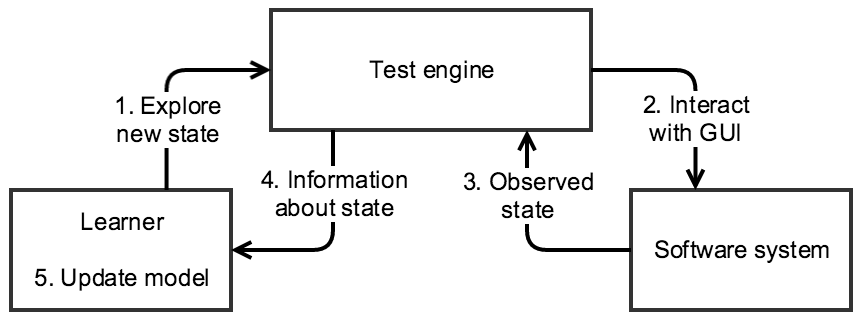
\includegraphics[width=0.9\linewidth]{figures/crawler.png}
    \end{center}

    \caption{The principle of inferring models with crawling
    techniques. The learner asks a test engine to stimulate the
	software under test through its GUI, and constructs a model
	using the information gathered by the test engine.}
    \label{fig:crawler}
\end{figure}

The works presented in this section originate from the automatic
testing of GUI applications, e.g., desktop, web, and more recently
mobile applications. As depicted in Figure \ref{fig:crawler},
models are generated by a learner that updates the model under
generation using events and states given by an automatic test
engine. This test engine stimulates the application through its
GUI (by triggering events, e.g., clicking on a button or a link),
and collects all the observed screens.  Screen after screen, the
application is explored (the technical term is: crawled) until
there is no more new screen to explore or until some conditions
(e.g., based on the processing time or the code coverage rate)
are satisfied. The collected events and screens are often
represented with transitions and states in a graph or state
machine, which expresses the functional behavior of the
application observed from its GUI. As the number of screens may
be infinite, some approaches require state abstractions to limit
the model size, and a few others merge equivalence states (the
equivalence relation being defined with regards to the context of
the application).

\begin{table}
	\begin{tabular}{| c | c | c | c | c | c | c |}

		\hline

		Paper &2& 3 & 4& 5 & 6 & 7 	\\
		\hline

		%\cite{monkey}                           &mobile                 &B  &  &IM &Random   & Yes	\\

		\cite{hungar2002}                       &distributed
        systems   &B  &  &FM&$\EuScript{L}^*$       & \\

		%\cite{Memon:2003}                        &desktop                &B  &  &M &DFS      &  \\

		\cite{5416728}                          &web                    &B  &  &  &Concolic & Yes \\

		\cite{concolicandroid12}                &mobile                 &W  &  &  &Concolic & 					\\

		\cite{Joorabchi:2012:REI:2420240.2420457}                    &mobile                 &B  &  &IM &DFS		& Yes 			 		\\

		\cite{webmate12}                        &web                    &B  &  &IM &         & Yes \\

		%\cite{dynodroid}                        &mobile                 &B  &Yes &  &Random 	& Yes		\\

		\cite{5954416,Amalfitano:2012:UGR:2351676.2351717}     &mobile                 &B  &  &IM &BFS DFS 	& Yes	\\

		\cite{guitar,MobiGUITARIEEESoftware2014}          &desktop, mobile        &B	&  &FM &DFS		& Yes  \\

		\cite{crawljax:tweb12}                  &web                    &B	&  &FM&Multiple &	\\

		\cite{4656395}                          &web                    &B 	&  &IM &DFS 		&   \\

		\cite{Choi2013}                         &mobile                 &B  &  &FM&DFS      &   \\

		\cite{WPX13}                            &mobile                 &G  &  &IM &Multiple(2)		& 	\\

		\cite{Azim13}                           &mobile                 &G	&Yes &IM &DFS		& Yes \\

		\cite{SP15}								&mobile                 &B	&Yes &FM &Multiple		& Yes \\
		\hline
	\end{tabular}
	\\

	\caption{An overview of some works on GUI application
	crawling. Column 2 represents the type of application under
	analysis. Column 3 indicated the accessibility (black-box
	(B), white-box (W), grey-box (G)). Column 4 gives whether the
	technique requires an external environment. Column 5
	indicates whether the technique builds formal models (FM) or
	non-formal models (IM). Column 6 gives the strategy or
	algorithm used to crawl the application. Last column (7)
	shows whether the technique handles potential crashes, i.e.
	errors encountered during crawling.}
	\label{table:gui_works}
\end{table}

All these approaches focus on different applications seen in
different viewpoints. We chose to summarize them in Table
\ref{table:gui_works}, considering the following features:

\begin{itemize}
	\item \textbf{Type of application and accessibility (col.
	2 and 3):} most of the approaches focus on desktop, web, or
	mobile applications. These applications share some common
	features, e.g., the events that can be applied on screens.
	Some papers focus on other kinds of systems though, e.g.,
	distributed and legacy systems \cite{hungar2002}.

	The accessibility refers to the information available and
	considered by a technique. Applications are often seen as
	black-boxes even though some authors prefer to consider
	white- or grey-boxes Column 3 in Table
	\ref{table:gui_works} indicates the accessibility chosen
	for each technique. For instance,
	\cite{concolicandroid12,5416728} present testing frameworks
	that exercise mobile applications and rely upon a
	systematic test generation technique, also known as concolic
	testing, to explore symbolic execution paths. These white-box
	approaches should theoretically offer a better code coverage
    than black-box automatic testing. In spite of that, the
    number of paths being explored concretely often limits to
    short paths only. Furthermore, the constraints have not to be
    too complex for being solved. As a consequence, the code
    coverage of these approaches is lower in practice.
	A few other works consider a grey-box perspective to reduce
	the exploration complexity. Azim et al. chose to apply static
	analyses on Android application source code to guide the
	application exploration \cite{Azim13}. Yang et al.
	\cite{WPX13} perform static analyses of Android application
	source code as well in order to list the available events
	that may be applied on screens;

	\item \textbf{Application environment (col. 4):} a few works
	\cite{Azim13,SP15} take the external environment (e.g., the
	operating system) of the GUI application into account.
	The approach proposed by Azim et al. \cite{Azim13} exercises
	Android applications with User Interface (UI) events but also
	with system events to improve code coverage. Examining
	application environments while testing is more complicated in
	practice, and it requires more assumptions on the
    applications. On the other hand, considering the application
    environment helps build more complete and accurate models
    \cite{SP15};


	\item \textbf{Model generation (col. 5):} all the approaches
	cited in Table \ref{table:gui_works} learn either formal
	(FM) or informal models (IM). Memon et al. \cite{guitar}
	introduced the tool \textit{GUITAR} for scanning desktop
	applications. This tool produces event flow graphs and trees
	showing the GUI execution behaviors. The tool
	\textit{Crawljax} \cite{crawljax:tweb12}, which is
	specialized in Asynchronous JavaScript and XML\footnote{A term and a technique that has been coined in 2005: \url{http://adaptivepath.org/ideas/ajax-new-approach-web-applications/}.} (AJAX) applications, produces state machine
	models to capture the changes of Document Object Model\footnote{\url{http://www.w3.org/DOM/}} (DOM)
	structures of web documents by means of events (click,
	mouseover,etc.).
	Amalfitano et al. proposed in
	\cite{Amalfitano:2012:UGR:2351676.2351717} a crawler that
	generates straightforward models, called GUI trees, only
	depicting the observed screens. In \cite{WPX13}, Yang et al.
	presented an Android application testing method that
	constructs graphs expressing the called methods. Salva and
	Laurençot proposed in \cite{SP15} a crawler of Android
	applications that infers Parameterized Labeled Transition
	Systems (PLTSs) capturing the UI events, the parameters used
	to fulfill screens, and the screen contents (widget
	properties).

	These models, and specifically the formal ones, offer the
	advantage to be reusable for Model-based methods
	(e.g., Model-based Testing and Verification methods).
	However, the model inference of GUI applications is often
	paired with the state space explosion problem. To limit the
	state space, these approaches
	\cite{MobiGUITARIEEESoftware2014,guitar,5954416,WPX13,SP15}
	require state-abstractions specified by users, given in a
	high level of abstraction. This choice is particularly
	suitable for comprehension aid, but it often implies a lack
	of information when it comes to generate test cases.
	Alternatively, some approaches try to reduce the model on
	the fly. The algorithms introduced in
	\cite{crawljax:tweb12,4656395} reduce the model size by
	concatenating identical states of the model under
	construction.  But this cannot be  applied on all
	applications in a generic manner since a state abstraction
	definition has to be (manually) given;

	\item \textbf{Exploration strategy (col. 6):} many
	papers propose at least one strategy to explore GUI
	applications. The Depth-First Search (DFS) is often
	considered since this strategy offers the advantage of
	resetting the application under test fewer time than any other
	strategy. Nonetheless, some works proposed different strategies
	\cite{Amalfitano:2012:UGR:2351676.2351717,5954416,crawljax:tweb12,WPX13}
	and demonstrated that it can either reduce the exploration
	time or help increase code coverage. In \cite{SP15}, Salva
	and Laurençot combined the Ant colony optimization heuristic
	with a model inference engine to support different kinds of
	exploration strategies. For instance, their algorithm
	supports semantics-based strategy, i.e. strategies guided by
	the content found in the application' screens;

	\item \textbf{Crash report (col. 7):} we define a crash as
	any unexpected error encountered by an application.  Crash
	reporting is another feature supported by some of the
	approaches in Table \ref{table:gui_works}.  When crashes
	are observed, reports are proposed to give the error causes
	and the corresponding application states. Furthermore, the
	methods proposed in
	\cite{MobiGUITARIEEESoftware2014,guitar,SP15} perform stress
	testing for trying to reveal more bugs,  for instance by
	using random sequences of events. The resulting models are
	completed thanks to these fault observations. In addition,
	the tool \textit{AndroidRipper}
	\cite{Amalfitano:2012:UGR:2351676.2351717} generates the test
	cases for each crash observed.

	Generally speaking, these techniques focus more on the GUI
	application exploration to detect bugs than on the model
	generation. For instance, a small number of algorithms consider state
	merging or the definition of state equivalence classes to
	reduce the model size. At the time of writing, only Choi et
	al. introduced an algorithm combining testing and the use
	of active learning \cite{Choi2013}. This algorithm is close
	to the approaches presented in Section
	\ref{sec:active-letoile}, but it also limits the number of
	times an application has to be reset. A testing engine, which
	replaces the teacher, interacts with the GUI application to
	discover new application states. The events and states are
	given to a learning engine that builds a model accordingly.
	If an input sequence contradicts the current model, the
	learning engine rebuilds a new model that meets all the
	previous scenarios.  This learning-based testing algorithm
	avoids restarts and aggressively merges states in order to
	quickly prune the state space. Consequently, the authors show
	that their solution outperforms the classical
	$\EuScript{L}^*$ technique but models are over-approximated.
	Salva and Laurençot also shown in \cite{SP15} that this
	approach requires much more time to build a model than the
	others.
\end{itemize}

Active inference approaches repeatedly query systems or humans to
collect positive or negative observations. Nonetheless, this can
lead to some issues like disturbing the system for instance. This
is not always suitable, and that is why another category of
methods infer models in a passive manner, i.e. without
stimulating the software system.  In the next section, we
introduce some of these passive model inference techniques.

%%%%%%%%%%%%%%%%%%%%%%%%%%%%%%%%%%%%%%%%%%%%%%%%%%%%%%%%%%%%%%%%%

\subsection{Passive model inference}
\label{sec:passive}

\begin{figure}[ht]
    \begin{center}
        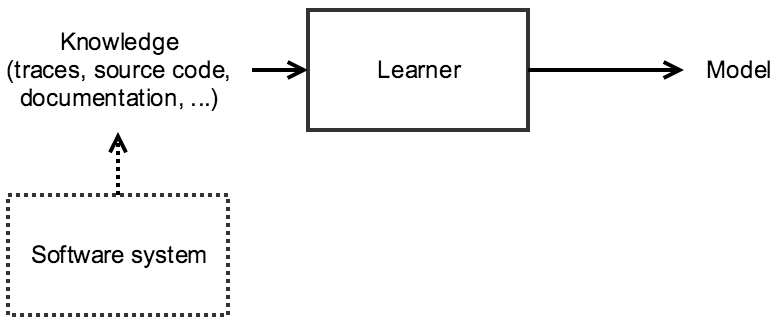
\includegraphics[width=0.9\linewidth]{figures/passive.png}
    \end{center}

    \caption{Passive model inference principle. The learner does
    not interact with the software system but rather relies on
    a fixed set of information (knowledge).}
    \label{fig:passive}
\end{figure}

The passive model inference category includes all techniques that
infer models from a fixed set of samples, such as a set of
execution traces, source code, or even documentation, as shown in
Figure \ref{fig:passive}. Since there is no interaction with the
system to model, theses techniques are said passive or offline.
In contrast to active model inference, the samples are usually
considered as positive elements. Also, models are often
constructed by initially representing sample sets with automata
whose equivalent states are merged. This section presents an
overview of these techniques.

A substantial part of the papers covering this topic proposes
approaches either based upon event sequence abstraction or
state-based abstraction to infer models. We introduce them in
Sections \ref{sec:passive-fsa} and \ref{sec:passive-spec}.
We present some white-box techniques, which retrieve
models from source code, in Section \ref{sec:passive-white}, as
well as a few alternative works leveraging documentation in
Section \ref{sec:passive-others}.

\subsubsection{Passive inference using event sequence abstraction}
\label{sec:passive-fsa}

Most of the following approaches, which build models from
execution traces by means of event sequence abstraction, are
build on-top of these two algorithms: \textit{kTail}
\cite{5009015} and \textit{kBehavior} \cite{mariani2007dynamic}.

kTail generates \textit{Finite State Automata} (FSA) from trace
sets in two steps. First, it builds a \textit{Prefix Tree
Acceptor} (PTA), which is a tree whose edges are labeled with
the event names found in traces. Then, kTail transforms the PTA
into a FSA by merging each pair of states as far as they exhibit
the same future of length $k$, i.e. if they have the same set of
event sequences having the maximum length $k$, which are all
accepted by the two states. This state merging step often yields
over-generalized models containing undesirable behaviors though
\cite{4023976}.

Reiss and Renieris modified the kTail algorithm to reduce the
size of the final FSA.  Indeed, their algorithm merges two states
if they share at least one \textit{k-future} \cite{919096}. By
using a merging criterion that is weaker, their variant actually
merges more states than kTail. Yet, the resulting FSA
express much more behaviors than those possible in the real
system. They are usually more approximate than the models
obtained with kTail. Lo et al. \cite{Lo:2009:ASB:1595696.1595761}
also enhanced the kTail algorithm to lower over-approximation.
Traces are mined to extract temporal properties that
statistically hold in most of the traces. Such temporal
properties aim at capturing relations between non consecutive
events. The kTail algorithm is then upgraded to prevent the
merging of states with the same k-future, which would produce FSA
that violate the inferred properties.

Lorenzoli et al. extended kTail to produce \textit{Extended
Finite State Machines} (EFSMs), which are FSMs extended with
parameters and algebraic constraints on transitions
\cite{Lorenzoli2008}. Their technique, called \textit{gkTail},
generates an EFSM from a set of traces, which incorporates
information about both the event sequences and the values of the
parameters associated with the event sequences. gkTail starts by
combining the traces that share the same event sequence, each
event being associated with the set of values obtained as the
union of all value assigned to this same event in each merged
trace. gkTail infers a constraint from the values associated with
each event, and combines this constraint with the associated
event. Finally, the kTail algorithm is applied on these traces.

\textit{kBehavior} \cite{mariani2007dynamic} is another
algorithm, which works quite differently than kTail. It generates
a FSA from a set of traces by taking every trace one after one,
and by completing the FSA such that it accepts the trace. More
precisely, whenever a new trace is submitted to kBehavior, it
first identifies the sub-traces that are accepted by sub-automata
in the current FSA (the sub-traces must have a minimal length
$k$, otherwise they are considered too short to be relevant).
Then, kBehavior extends the model with the addition of new
branches that connect the identified sub-automata,
producing a new version of the model that accepts the entire
trace. They successfully applied this algorithm to automatically
analyze log files and retrieved important information to identify
failure causes \cite{4700316}. They also automatically analyzed
logs obtained from workloads to highlight useful information that
can relate the failure to its cause
\cite{cotroneo2007investigation}. Both works
\cite{4700316,cotroneo2007investigation} use an extended version
of kBehavior, called \textit{kLFA}, that supports events
combined with data values. kLFA performs a preliminary step by
analyzing the traces to infer parameter constraints. It encodes
these constraints in the event names with specific symbols to
yield new traces. kBehavior is then called to infer a FSA whose
transitions are still labeled with an event and a symbol
representing a data constraint.

Lo et al. presented an empirical comparative study of kTail,
kBehavior, gkTail, and kLFA with a set of 10 case studies
extracted from real software systems in \cite{Lo20122063}. This
study quantifies both the effect of adding data flow information
within automata and the effectiveness of the techniques when
varying sparseness of traces. One of the main conclusions is that
adding algebraic constraints to FSA does not compromise quality
but negatively affects performance. This is the case for gkTail
for instance, which becomes extremely slow. The study also
revealed that increasing the trace set improves the rate of
correct behaviors in models, especially for kTail and kBehavior.
But increasing the trace set does not particularly affect illegal
behavior rates, i.e. the number of behaviors found in the models
but not in the traces. This can be explained by the fact that
these algorithms are not really able to control
over-generalization when only positive samples are available. A
comparison has also be made between the kTail- and
kBehavior-based methods. In short, kTail provides low illegal
behavior rate, but also low correct behavior rate. On the other
hand, kBehavior has higher illegal behavior rate, but good
correct behavior rate.

The next section gathers the approaches building models from
traces that also consider invariants to merge states.

\subsubsection{Passive inference using state-based abstraction}
\label{sec:passive-spec}

The approaches presented in this section rely on the generation
of state invariants to define equivalence classes of states that
are combined together to form final models. The \textit{Daikon}
tool \cite{Ernst:1999:DDL:302405.302467} was originally proposed
to infer invariants composed of data values and variables found
in execution traces. An invariant is a property that holds at a
certain point or points in a software. These are often used in
assert statements, documentation, and formal specifications. An
invariant generator mines the data found in the traces that a
software system produces, and then reports properties that are
$true$ over the observed executions.  This is a machine learning
technique that can be applied to arbitrary data. Daikon is used
in many different kinds of works, e.g., for generating test cases,
predicting incompatibilities in component integration, automating
theorem proving, repairing inconsistent data structures, and
checking the validity of data streams, among other tasks
\cite{Ernst200735}.

Krka et al. inferred object-level behavioral models (FSA) from
object executions, by using both invariants, representing object
states, and dynamic invocation sequences, expressing method
invocations \cite{Krka:2010:UDE:1810295.1810324}.
Invariants are still generated with Daikon. The authors show that
their FSA inference technique offers more precise models than
those obtained with kTail, which means that the rate of
over-approximation is lower. These results are not surprising
since they use a state merging technique combining event sequence
abstraction and state abstraction. Hence, state merging is here
done with more precision.

In \cite{Ghezzi:2009:SIB:1555001.1555057}, Ghezzi et al.
described an approach called \textit{SPY} to recover a
specification of a software component from its traces. They infer
a formal specification of stateful black-box components (Java
classes that behave as data containers with their own states).
Model inference is performed in two main steps. It starts by
building a DFA that models the partial behavior of the instances
of the classes. Then, the DFA is generalized via graph
transformation rules that are based upon the following
assumption: the behavior observed during the partial model
inference process benefits from the so called "continuity
property" (i.e. a class instance has a sort of "uniform"
behavior). Transformation rules generate data constraints that
hold for each encountered data value found in the instance pools.
Such constraints add over-approximation to the model though.

Walkinshaw et al. presented the \textit{Query-driven State
Merging} (QSM) algorithm in
\cite{Walkinshaw07reverseengineering}, an \textit{interactive}
grammar inference technique to infer the underlying state machine
representation of software. The QSM algorithm does not infer
invariants but uses the Price's "blue-fringe" state merging
algorithm \cite{Lang:1998:RAO:645517.655780}, which is mainly
based upon fixed invariants defining order relations over states.
QSM generalizes a supplied trace set obtained from an application
by applying two steps: (i) a trace abstraction is performed
with functions given by a user, and (ii) states are merged with
the Price's "blue-fringe" state merging algorithm. To avoid
over-generalization, the algorithm queries the user whenever the
resulting machine accept or reject sequences that have not
been ratified. This approach can be compared to the work done by
Hungar in \cite{hungar}, who used the $\EuScript{L}^*$ algorithm
instead. But the QSM algorithm presumes that the input sequences
offer some basic coverage of the essential functionality of the
system, in which case the machine can be inferred relatively
cheaply by a process of state merging, compared to the
$\EuScript{L}^*$ technique that systematically and
comprehensively explores the state space of the target machine.
Some tools such as \textit{Synapse}
\cite{LamelaSeijas:2014:SAB:2633448.2633457} implement the QSM
algorithm to perform automatic behavior inference and
implementation comparison for the programming language Erlang.

Taking another direction by leveraging genetic algorithms,
Tonella et al. \cite{TonellaNMLH13} applied a data-clustering
algorithm to infer FSMs from traces. Traces are transformed into a
first FSM where every state is considered as one distinct
equivalence class, called cluster. Then, invariants are generated
with Daikon for each cluster in order to group states. The
clustering is iteratively improved by using a genetic algorithm
that randomly update the clusters. But the clustering is yet
guided with the computation of quality attributes on the current
FSM model. Each distinct set of invariants produced for each
cluster at the end of the optimization represents an abstract
state, and is used as the abstraction function that maps states
to more abstract ones. Even though this approach offers
originality, it is time consuming, especially with a large set of
traces.

The works presented in this section adopted either a grey- or
black-box approach. The next section introduces some white-box
techniques.

\subsubsection{White-box techniques}
\label{sec:passive-white}

The works presented in this section adopt a white-box
perspective. Models are built by following two different
procedures: (i) the source code is instrumented and the system is
executed or tested to collect traces from which a specification
can be generated, and (ii) the source code is statically analyzed
to directly infer models.

Ammons et al. reuse the kTail algorithm to produce
non-deterministic automata from source code
\cite{Ammons:2002:MS:565816.503275}. The latter is instrumented
to collect the function calls and parameters.  Application traces
are collected and scenarios (small sets of interdependent
interactions) are then derived. kTail is finally employed to
build automata. Several automata are generated from the different
scenarios.

Whaley et al. suggested to use multiple FSM submodels to model
object-oriented component interfaces
\cite{Whaley:2002:AEO:566171.566212}. A FSM is built for each
attribute of a class, with one state per method that writes that
attribute. The FSMs are reduced with restrictions on the methods:
a distinction is made between side-effect-free methods, i.e. those
that do not change the object state, and the others. The
side-effect-free methods are ignored to build FSMs. The others are
completed with dotted transitions to represent the states
from which it is possible to call these side-effect-free methods.
Two techniques are given to automatically construct such models:
(i) a dynamic instrumentation technique that records real method call
sequences, and (ii) a static analysis that infers pairs of
methods that cannot be called consecutively. The work described
in \cite{Alur:2005:SIS:1047659.1040314} generates behavioral
interface specifications from Java classes by means of predicate
abstraction and active learning. This is a white-box approach
inspired by \cite{Whaley:2002:AEO:566171.566212} that, first,
uses \textit{predicate abstraction} to generate an abstract
version of the considered class. Afterwards, a minimal version
(interface) of this abstraction is constructed by leveraging the
$\EuScript{L}^*$ algorithm. The tool \textit{Java Interface
Synthesis Tool} (JIST) is the resulting implementation of such a
technique. It takes Java classes as input, and generates useful
and safe interfaces automatically.

Still in the purpose of modeling object invocation, Salah et al.
proposed \textit{Scenariographer} \cite{Salah05scenariographer},
an algorithm and a tool to estimate the usage scenarios of a
class from its execution profiles. The results are quite
different than the above approaches tough, since Scenariographer
infers a set of regular expressions expressing the generalized
usage scenarios of the class over its methods. The source code is
still instrumented to collect method calls, but this approach
employs the notion of canonical sets to categorize method
sequences into groups of similar sequences, where each group
represents a usage scenario for a given class.

Yang et al. \cite{Yang:2006:PMT:1134285.1134325} also focused on
the model inference of Java programs but they use a state
abstraction technique generating temporal invariants. The source
code is instrumented to collect method invocations. Then,
temporal invariants are extracted to capture relations among
several consecutive or non-consecutive events. The resulting tool
\textit{Perracotta} infers temporal invariants and FSMs from
traces. It is able to scale to large software systems since it
can infer models from millions of events. Additionally, it works
effectively with incomplete trace sets typically available in
industrial scenarios. Scalability is here obtained by the use of
heuristics to prune the set of inferred invariants.

In \cite{Pradel:2009}, Pradel and Gross presented a scalable
dynamic analysis that infers extremely detailed specifications of
correct method call sequences on multiple related objects. Again,
Java applications are executed to collect with debuggers methods
calls. This produces a large set of traces. Given that methods
generally implement small and coherent pieces of functionality,
the source code is statically analyzed to identify small sets of
related objects (object collaborations), and method calls that
can be analyzed separately. Then, they derive FSMs that model
legal sequences of method calls on a set of related objects. This
work has been extended in \cite{Dallmeier_generatingtest} by
means of active testing. The inference engine generates the test
cases that cover previously unobserved behaviors, systematically
extending the execution space and enriching the models while
detecting bugs. Such an approach is similar to the crawling
techniques presented in Section \ref{sec:active-crawling} except
that crawlers take GUI applications as input.

Even though the remaining papers are oriented towards the same
purpose, that is model inference from source code, they do not
collect traces from executions but perform static analysis only.
Shoham et al. introduced an approach to infer finite automata
describing method calls of an API from source code of the client
side, i.e. the code that calls the API
\cite{Shoham:2007:SSM:1273463.1273487}. Finite automata are
constructed with two main steps: (i) abstract-traces are
collected with a static analysis of the source code and split
into sets called abstract histories that give birth to several
finite automata, and (ii) a summarization phase filters out
noise. This step is done thanks to two available criteria: either
all the histories are considered (no filter) or the histories
having the same k-future (as with kTail) are assembled together.
Despite encouraging results, the inferred specifications are
often too detailed, and their solution does not scale well.

In \cite{Wasylkowski07detectingobject}, Wasylkowski et al.
proposed \textit{JADET}, a Java code analyzer to infer method
models. One finite state automaton is built for every class to
express the method calls. JADET then infers temporal properties
grouped into patterns that can be used to automatically find
locations in programs that deviate from normal object usage.
Temporal properties are obtained by the use of the data mining
technique frequent itemset mining, which is applied on the source
code. These properties are fed into a classifier that detects and
removes the abnormal properties. It then identifies the methods
that violate the remaining ones.

The next section introduces a few other works leveraging
documentation to infer models.

\subsubsection{Model inference from documentation}
\label{sec:passive-others}

We present in this section some other passive inference
techniques that rely on other sets of knowledge to infer models.
Their main disadvantage lies in the use of external documentation
that can be outdated, leading to models describing incorrect
behaviors (over-approximation). Furthermore, the resulting models
are often under-approximated since documentation is usually not
complete. That is probably why there are few works based on
documentation mining in the literature.

Bertolino et al. presented \textit{StrawBerry} in
\cite{Bertolino:2009:ASB:1595696.1595719}, a method that infers a
Behavior Protocol automaton from a Web Service Description
Language (WSDL) document.  WSDL is a format for documenting web
service interactions, containing information about the inputs,
outputs, and available methods. StrawBerry automatically derives a
partial ordering relation among the invocations of the different
WSDL operations, that is represented as an automaton called
Behavior Protocol automaton.  This automaton models the
interaction protocol that a client has to follow in order to
correctly interact with a web service.  The states of the
behavior protocol automaton are web service execution states, and
the transitions, labeled with operation names and input/output
data, model possible operation invocations from the client to the
web service.

Later, Zong et al. \cite{ZhongZXM11} proposed to infer
specifications from API documentation to check whether
implementations match it. A linguistic analysis is applied as API
documentation is written in a natural language. It results in a
set of methods that are linked together with action-resource
pairs that denote what action the method takes on which resource.
Then, a graph is built from these methods and a predefined
specification template. Such specifications do not reflect the
implementation behaviors though. Furthermore, this method can be
applied only if the API documentation is available in a readable
format, and if a specific template is provided.

In the sequel, we present two approaches combining model
inference and expert systems to infer models from traces for web
applications (Chapter \ref{sec:modelinf:webapps}) and industrial
systems (Chapter \ref{sec:modelinf:prodsystems}). The state
merging is replaced with a context-specific state reduction based
on an event sequence abstraction. This state reduction can be
seen as the kTail algorithm introduced previously where $k$ is as
high as possible. Furthermore, our work focus on both speed and
scalability to be able to construct models of Michelin's
production systems in an efficient manner. Among all potential
use cases, we need such models to perform passive testing on
these production systems.
